\chapter{More information from TEM and EDX experiments}
\label{chapter:appendix_TEM}
We measured TEM together with EDX to get information on the chemical composition of sample S$_\mathrm{cap}$. The results shown in Fig.~\ref{fig:TEM_app} confirm the constituents given in Fig.~\ref{fig:TUstructure}.


\begin{figure}
	\centering
	\includegraphics[width=0.77\linewidth]{/TEM/TEM_appendix/TEM_12040}
	\caption{(a) TEM image measured under bright field conditions using the (200) reflection perpendicular to the growth direction. (b) EDX map in Al which is present only in Al$_{0.4}$GaP layer.}
	\label{fig:TEM_app}
\end{figure}

The emission EDX spectrum (Fig.~\ref{fig:EDX}) shows all elements present in S$_\mathrm{cap}$ sample, i.~e., Ga, P, In, As, Sb, Al; oxygen is detected due to degradation of the sample by oxidation processes; Co, Fe and Zr are typical compounds used in TEM objectives. In Fig.~\ref{fig:concentration_appendix} the distribution of the concentration in the vertical cut is shown, Al$_{0.4}$GaP layer and QD areas are located between 250 and 280$\,$nm and around 80$\,$nm, respectively.
\begin{figure}
	\centering
	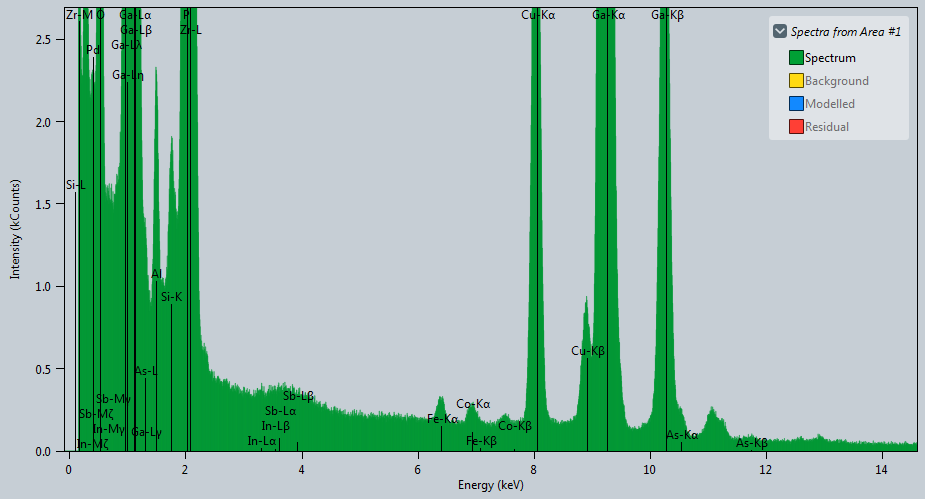
\includegraphics[width=0.77\linewidth]{/TEM/TEM_appendix/EDX}
	\caption{EDX spectrum measured on S$_\mathrm{cap}$.}
	\label{fig:EDX}
\end{figure}


\begin{figure}
	\centering
	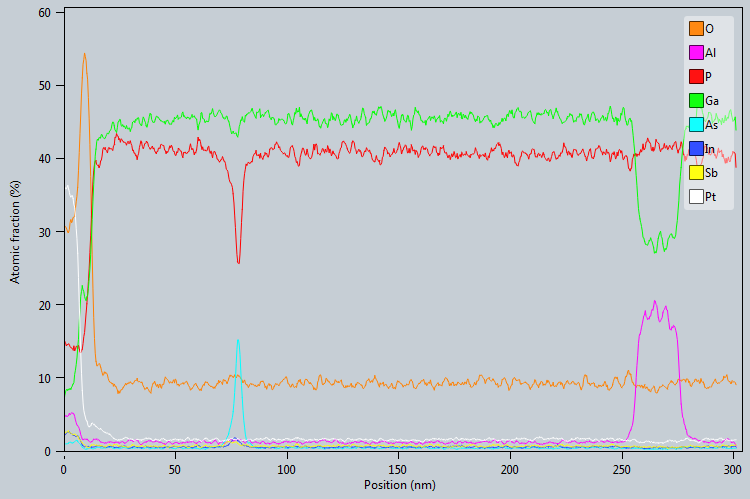
\includegraphics[width=0.77\linewidth]{/TEM/TEM_appendix/concentration}
	\caption{Atomic fraction as a function of position in the vertical cut (the zero position is associated with the surface of the sample).}
	\label{fig:concentration_appendix}
\end{figure}

\newpage 